\section{Speckle}
\begin{figure}[ht]
\centering
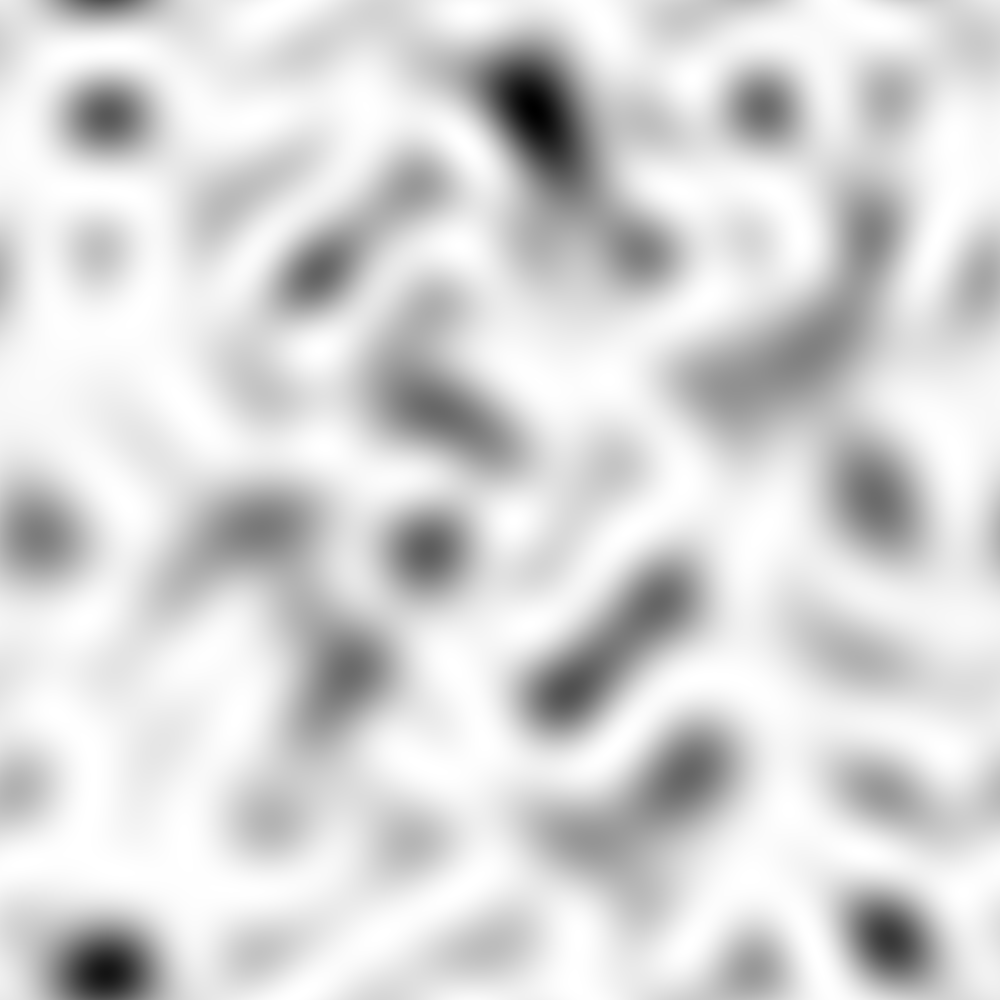
\includegraphics[width=5cm,keepaspectratio]{figures/speckle.png}
\caption{Example speckle field produced by the Fourier transform method.}
\end{figure}
When coherent waves with randomly distributed phases and amplutudes
interfere, the result exhibits seemingly random intensity fluctuations
known as \textit{speckle}.  


\section{Statistical Properties}
To begin, we assume the field at each detector position $E(\mathbf{r})$ is
due to the coherent linear superposition of $N$ random phasors
\begin{equation}
E(\mathbf{r}) = \frac{1}{\sqrt{N}} \sum_{n=1}^{N} a_n \me^{\mi \phi_n}
\end{equation}
where the amplitude of the $n$th phasor is $a_n$ and its phase $\phi_n$ is
randomly distributed on the interval $(-\pi,\pi)$.  In reality, these
conditions may be loosened by the physics of the actual experiment, which
we will describe later.

By the central limit theorem, as $N\to\infty$, the resultant probability
distribution $p_E(E)$ of $E(\mathbf{r})$ is Rayleigh distributed and the
corresponding probability distribution $p_I(I)$ of the intensity
$I(\mathbf{r})=|E(\mathbf{r})|^2$ is an exponential
\begin{equation}
p_I(I) = \frac{1}{2\sigma_I^2}\exp\left(-\frac{I}{2\sigma_I^2}\right)
\label{eqn:propexp}
\end{equation}

Because the $q$th moment of $p_I(I)$ is given by 
\begin{align}
\bar{I}^q&=(2\sigma_I^2)^q q!\\
         &=\bar{I}^q q!
\end{align}
we see that the standard deviation of is equal to the mean: 
$\sigma_I=\bar{I}$.  \Equation{eqn:propexp} can then be rewritten
\begin{equation}
p_I(I) = \frac{1}{\bar{I}}\exp\left(-\frac{I}{\bar{I}}\right)
\end{equation}

called fully developed speckle
The fact that the 

\begin{figure}
\centering
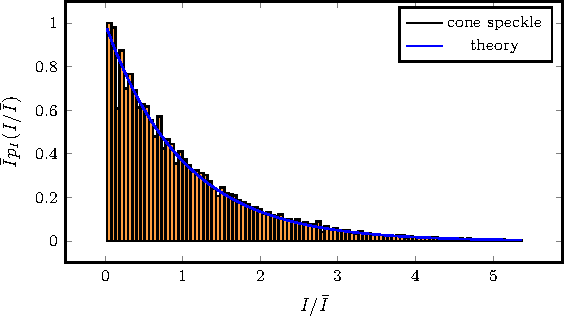
\includegraphics[keepaspectratio]{figures/spk_ihist.pdf}
\caption{Cone speckle: negative exp vs guy}
\end{figure}

\subsection{Small Number of Scatterers}
\begin{equation}
p_I(I) = 2\pi^2 \int_0^\infty\! \rho J_0\!\left(\frac{2\pi a
\rho}{\sqrt{N}}\right)^N J_0\!\left(2\pi\sqrt{I}\rho\right)\md\rho
\end{equation}
with $\rho_I^2=(1-1/N)a^4$.

single scattering
contrast

\section{Spatial Correlations}


